
\documentclass{article}

%encoding
%--------------------------------------
\usepackage[utf8]{inputenc}
\usepackage[T1]{fontenc}
%--------------------------------------

\usepackage{geometry}
\usepackage{amsmath}
\usepackage{graphicx}
\usepackage{float}

\usepackage[brazilian]{babel}
\usepackage{hyphenat}
\hyphenation{mate-mática recu-perar}

 \geometry{
 a4paper,
 total={170mm,257mm},
 left=20mm,
 top=20mm,
 }

\title{Relatório do trabalho 4}
\date{10/06/2019}
\author{Allan Nozomu Fukasawa RA:163527}

\begin{document}
\maketitle

\section{Introdução}

O objetivo deste trabalho é aplicar técnicas de detecção de pontos de interesse para, a partir de um par de imagens, criar uma imagem panorâmica pela ligação entre os pontos de interesse, formando uma correspondência.

Os passos seguidos para a execução do trabalho foram extraídos de sua especificação. \cite{Helio:1}

\section{Componentes}

Está sendo enviado junto a este relatório os seguintes arquivos e diretórios:

\begin{itemize}
  \item arquivo Trabalho 4.ipynb: contém todo o código executado durante este trabalho.

  \item quatro imagens utilizadas durante o processamento (todas disponíveis pelo professor no seguinte link \textit{http:\/\/www.ic.unicamp.br/\~helio\/imagens\_registro\/}. No arquivo do Jupyter Notebook, está sendo utilizada as imagens \textit{foto4A.jpg} e \textit{foto4B.jpg}, as imagens respectivamente \ref{Fig:imagemA} e \ref{Fig:imagemB}.

  \item resultados em formato de imagem, tanto a imagem final (panorâmica) quanto a imagem de relação entreos pontos em comum entre as duas imagens respctivamente as imagens \ref{Fig:resultado} e \ref{Fig:relacao}.
\end{itemize}

\begin{figure}[!htb]
  \begin{minipage}{0.48\textwidth}
    \centering
    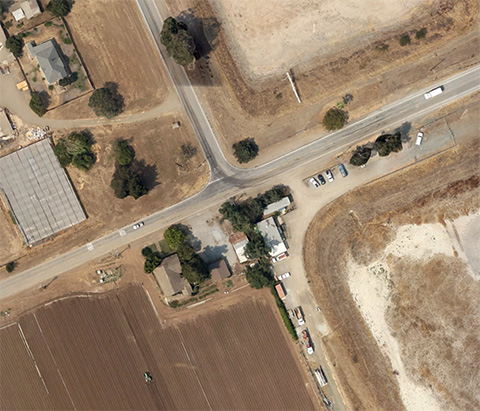
\includegraphics[width=.99\linewidth]{images/foto4A.jpg}
    \caption{Imagem A}\label{Fig:imagemA}
  \end{minipage}\hfill
  \begin{minipage}{0.48\textwidth}
    \centering
    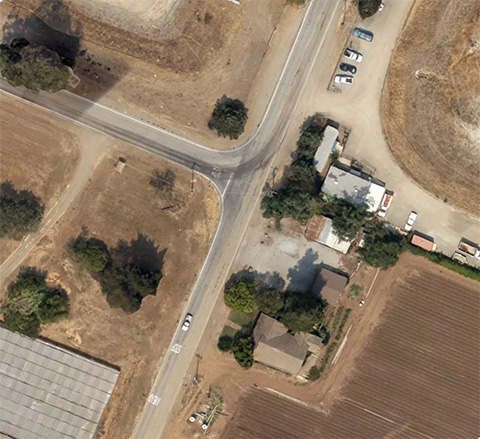
\includegraphics[width=.99\linewidth]{images/foto4B.jpg}
    \caption{Imagem B}\label{Fig:imagemB}
  \end{minipage}
\end{figure}

\subsection{O Programa}

O programa foi implementado com Jupyter Notebooks, usando Python 3.7.1. As bibliotecas utilizadas no desenvolvimento do programa foram, com suas respectivas versões: 

\begin{itemize}
    \item numpy (1.15.4): para manipulação dos vetores.

    \item matplotlib (3.0.2): visualização dos dados, resultados finais e intermediários.

    \item opencv (3.4.2): realização da leitura e escrita das imagens, transformação das cores (tanto em escala de cinxa quanto na coloração de RGB para BGR).

\end{itemize}

\subsection{Formato das imagens}

As imagens de entrada estão no formato .jpg. As imagens de saída, tanto as finais quanto as intermediárias se encontram no formato .jpeg.

\section{Leitura, escrita e plotagem das imagens}

\subsection{Leitura das imagens}

A imagem de entrada é lida com função \textbf{cv2.imread} que armazena a imagem em um \textbf{numpy.ndarray} de 3 dimensões (MxNx3).

Depois de lida, uma cópia da imagem é convertida para níveis de cinza pela função \textbf{cv2.cvtColor}, pois os algoritmos de detecção de pontos de interesse tem de estar em escala de cinza. A imagem original também teve que sofrer mudanças quanto a conversão de cores, pois por padrão, o OpenCV lê a imagem e armazena-a em formato de cores BGR. Portanto, foi-se utilizado a conversão para RGB para visualização dos dados usando matplotlib e depois convertida novamente para BGR na hora de savar os resultados.

\subsection{Escrita das imagens}

Também foi feito uma função auxiliar para facilitar na saída das imagens utilizando a função \textbf{cv2.imwrite}. Assim como dito anteriormente, antes de salvar as imagens, foi convertida novamente do formato RGB para BGR.

\subsection{Plotagem das imagens}

Foi utilizado para visualização dos resultados as funções de plotagem de imagens em \textbf{matplotlib.pyplot}.

\section{Solução}

\subsection{Pontos de interesse}

 Para a detecção dos pontos de interesse das imagens, primeiramente foi-se convertida em escala de cinza. Depois, foram utilizadas 3 algoritmos diferentes, sendo todos apresentando resultados bem similares:

 \begin{itemize}
  \item SIFT (Scale Invariant Feature Transform): utilizando \textit{cv2.xfeatures2d.SIFT\_create()}
  

  \item SURF (Speed Up Robust Feature): utilizando \textit{cv2.xfeatures2d.SURF\_create()}
  
  \item ORB (OrientedFAST, Rotated BRIEF).): utilizando \textit{cv2.ORB\_create()}

\end{itemize}

Depois de identificado cada um dos pontos de interesse, foi-se computado as distâncias (similariedades) entre cada descritor das duas imagens. Para isso, utilizou-se uma correspondência utilizando um método de força bruta, onde para cada ponto é verificato a distância euclidiana entre todas as features  e verifica-se qual é o par que apresenta a menor distância.

Além disso, é aplicado o algoritmo de KNN (K-Nearest Neighbours), com 2 vizinhos para verificar se a distância esta no limiar e também para evitar pontos falso-positivos. Depois, para cada relação, é aplicado o teste de relação de Lowe. No caso, foi-se utilizado um fator de correspondência de 0.75.

Depois, caso tenha-se encontrado ao menos 4 pontos de interesse em comum, é calculado a matrix de Homografia, utilizando a função do opencv \textit{findHomography} e passando os pontos como parâmetro bem como a técnica empregada que foi a RANSAC (RANdom SAmple Consensus).

Nota-se que há uma limitação na solução apresentada em que a correspondência e também a formação da imagem panorâmica foi só possível ser realizada a partir da imagem da esquerda para a imagem da direita.

\subsection{Resultados}

Seguindo os passos, foi-se estimada a seguinte matriz de homeografia:

\begin{center}
  $
  \begin{bmatrix}

    1.15562971+00 & 1.09434802+00 & -2.19606581+02 \\ 
 
    -1.09444476+00 & 1.15562133+00 & 2.12948548+02 \\ 
 
    5.29573677-07 &  2.21007038-07 & 1.00000000+00 \\ 
 
  \end{bmatrix}
  $
\end{center}

Além disso, utilizando a função \textit{drawMatchesKnn} foi possível desenhar os pontos de correspondência entre as duas imagens disponíveis na imagem \ref{Fig:relacao} obtidos através das correspodências obtidas.

\begin{figure}[!htb]
  \centering
  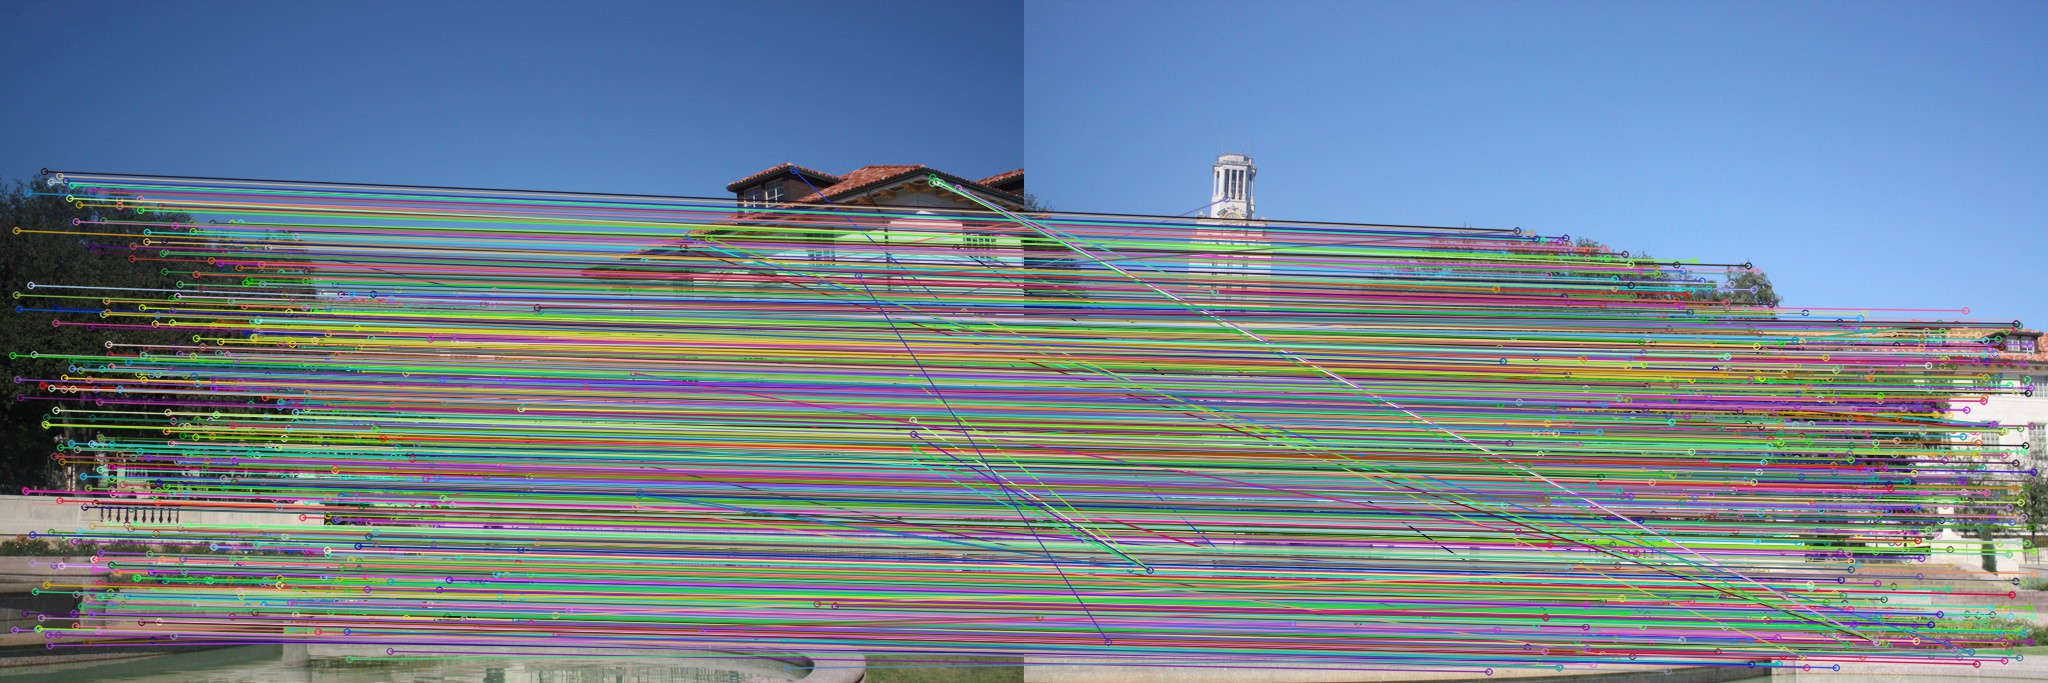
\includegraphics[width=.8\linewidth]{relation.jpeg}
  \caption{Linhas de correspondência entre as duas imagens, utilizando-se SURF}\label{Fig:relacao}
\end{figure}

Utilizando a função \textit{warpPerspective} foi possível também unir as duas imagens formando uma panorâmica. Para isso, primeiramente a imagem a direita foi desenhada em uma imagem resultante de no maximo a soma das duas larguras e a maior altura. Depois, sobreescreveu-se a imagem a esquerda, obtendo o resultado da imagem \ref{Fig:resultado}

\begin{figure}[!htb]
  \centering
  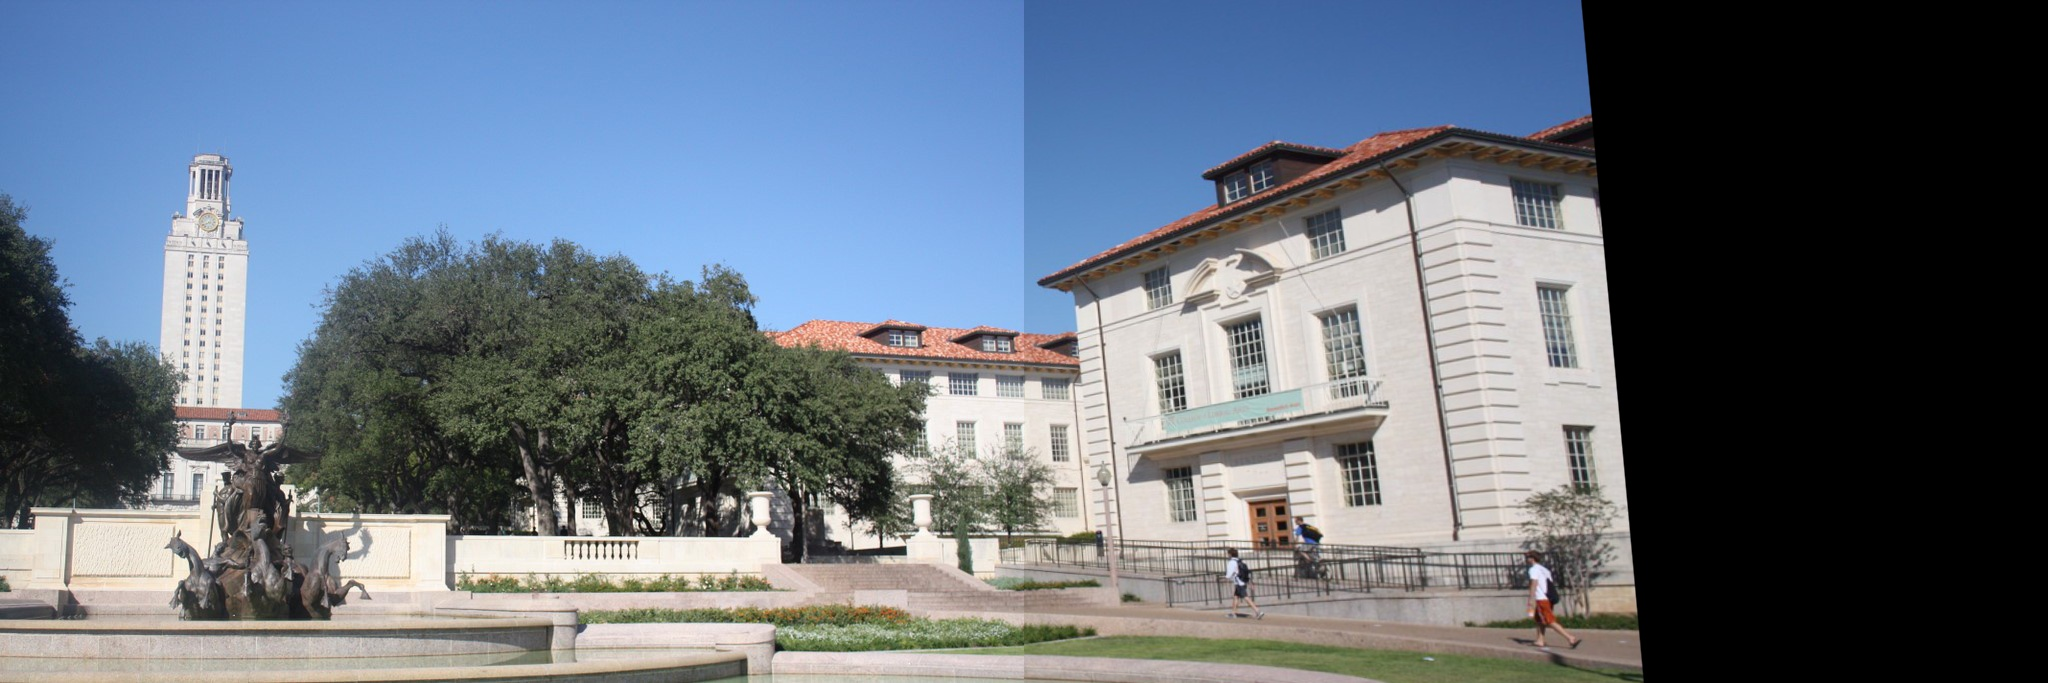
\includegraphics[width=.8\linewidth]{result.jpeg}
  \caption{Resultado da imagem panorâmica formada pelas duas imagens}\label{Fig:resultado}
\end{figure}

\section{Conclusão}

Após a execução de todos os procedimentos foi possível formar a imagem panorâmica, mas com a limitação de formar a imagem da esquerda para a direita. Sendo assim, apenas é possível sobreescrever uma imagem sobre a outra e não o contrário.

Podemos perceber que, tanto no SIFT quanto no SURF, o número de pontos por padrão foi substancialmente maior do que o do ORB. Porém é possível alterar adicionando novos parâmetros para a detecção de novos pontos de interesse no ORB. Porém, em todos, os números de pontos foi suficiente para se realizar a imagem panorâmica e também para o cálculo da matriz de homogrfia.

Além disso, as imagens a serem unidas podem apresentar diferentes contrastes, níveis de brilho e cores, o que leva a clara detecção da união das imagens. Portanto, para melhores resultados, ainda é necessário fazer um pós processamente para nivelar os níveis de cores e contrastes principalmente na união entre elas.

\bibliography{relatorio4}
\bibliographystyle{ieeetr}

\end{document}